\chapter{Results and Discussion}

From a molecular perspective, circRNAs are similar to their linear
counterparts, with the primary distinction being their circular structure.
As explained in \cref{sec:circrna_biogenesis}, circRNAs are derived from a
linear precursor (identical to linear RNA) that undergoes back-splicing to form
a loop.
Thus, the only way to computationally identify circRNAs is by detecting reads
spanning the back-splice junction (BSJ), which cannot be accounted for by
canonical forward splicing.
Several tools for BSJ detection are discussed in
\cref{subsec:circrna_detection}.

However, detecting BSJs only pinpoints the start and end of a circRNA within
the genome, without revealing its internal structure.
To reconstruct the full circRNA sequence, a de novo assembly of the circular
transcriptome that accounts for back-splice junctions is required.
Tools like CIRI-full, circRNAfull, and JCcirc are capable of this task, but
they rely on paired-end or long-read sequencing data.
To date, no tools are available for de novo assembly of circRNAs using
single-end short-read data.
Since the data used in this thesis is single-end, the focus is limited to the
detection, quantification, and analysis of BSJs.

\section{Back-splice junction (BSJ) detection}

For detection of BSJs, five different detection tools were used: circexplorer2,
ciriquant, dcc, find\_circ and segemehl.
While the nf-core/circrna pipeline provides a wider selection of tools, these
are the only ones which work with single-end sequencing data.

\begin{figure}[ht]
    \begin{tabular}{cc}
        \begin{subfigure}{.5\textwidth}
            \centering

            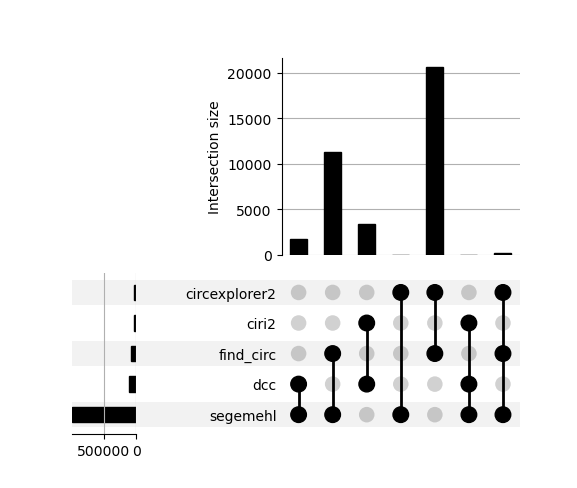
\includegraphics[width=\linewidth]{chapters/4_results_and_discussion/figures/detection/upset/diff_0_strand.png}
            \caption{No shift allowed, strand considered}
            \label{fig:detection_upset_full}
        \end{subfigure}
         &
        \begin{subfigure}{.5\textwidth}
            \centering

            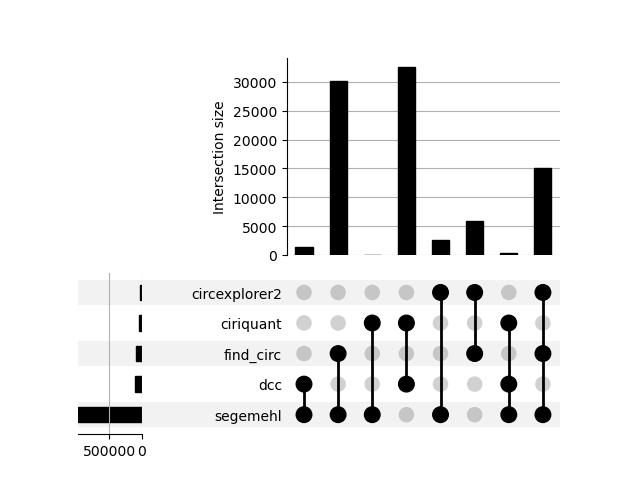
\includegraphics[width=\linewidth]{chapters/4_results_and_discussion/figures/detection/upset/diff_0_nostrand.png}
            \caption{No shift allowed, strand ignored}
            \label{fig:detection_upset_nostrand}
        \end{subfigure} \\
        \multicolumn{2}{c}{
            \begin{subfigure}{\textwidth}
                \centering

                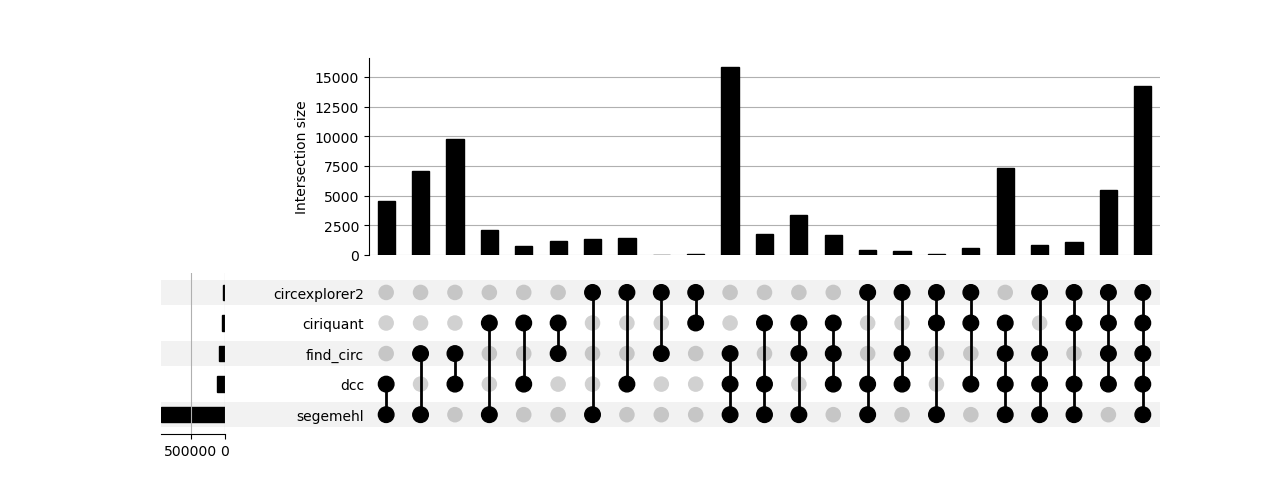
\includegraphics[width=\linewidth]{chapters/4_results_and_discussion/figures/detection/upset/diff_1_nostrand.png}
                \caption{Shift of 1 allowed, strand ignored}
                \label{fig:detection_upset_microshift}

            \end{subfigure}}
    \end{tabular}
    \caption{Upset plots showing the overlap of BSJs detected by different
        tools using various grouping criteria.
        Only groups with at least two agreeing tools are displayed.
        When considering strand information and only counting BSJs with identical start
        and end positions, many BSJs are detected by just two tools, with very few
        detected by three tools (\cref{fig:detection_upset_full}).
        Ignoring the strand information substantially increases the number of BSJs
        detected by 3 tools (\cref{fig:detection_upset_nostrand}).
        Allowing a shift of 1 bp in the start and end positions while ignoring the
        strand information changes the results drastically, leading to a large number
        of circRNAs with agreement between 4 and even 5 tools
        (\cref{fig:detection_upset_microshift}).
    }
    \label{fig:detection_upset}
\end{figure}

\begin{figure}[ht]
    \centering

    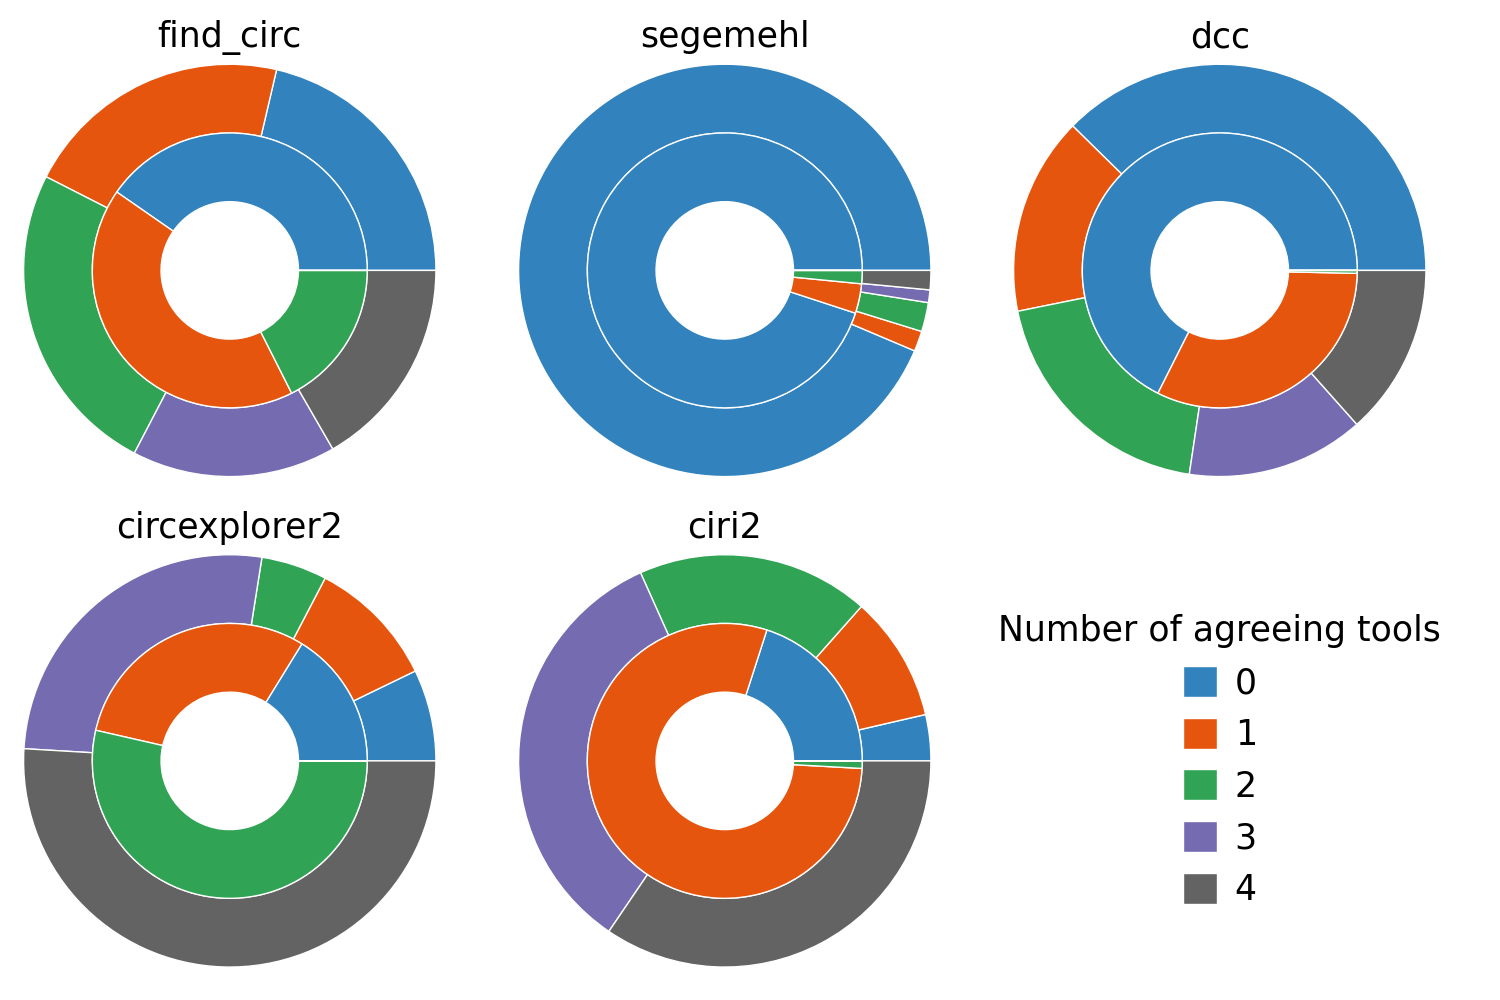
\includegraphics[width=0.7\textwidth]{chapters/4_results_and_discussion/figures/detection/pies.png}
    \caption{Pie charts showing the agreement of each tool with the others.
        The inner circle shows the agreement without allowing a shift in the start and
        end positions, while the outer circle shows the agreement when allowing a shift
        of 1 bp.
        While find\_circ, dcc, circexplorer2, and ciriquant behave similarly, segemehl
        detects a much larger number of BSJs, with a large portion of them not being
        detected by any other tool.
    }
    \label{fig:detection_pies}
\end{figure}

\begin{figure}[ht]
    \begin{tabular}{cc}
        \begin{subfigure}{.5\textwidth}
            \centering

            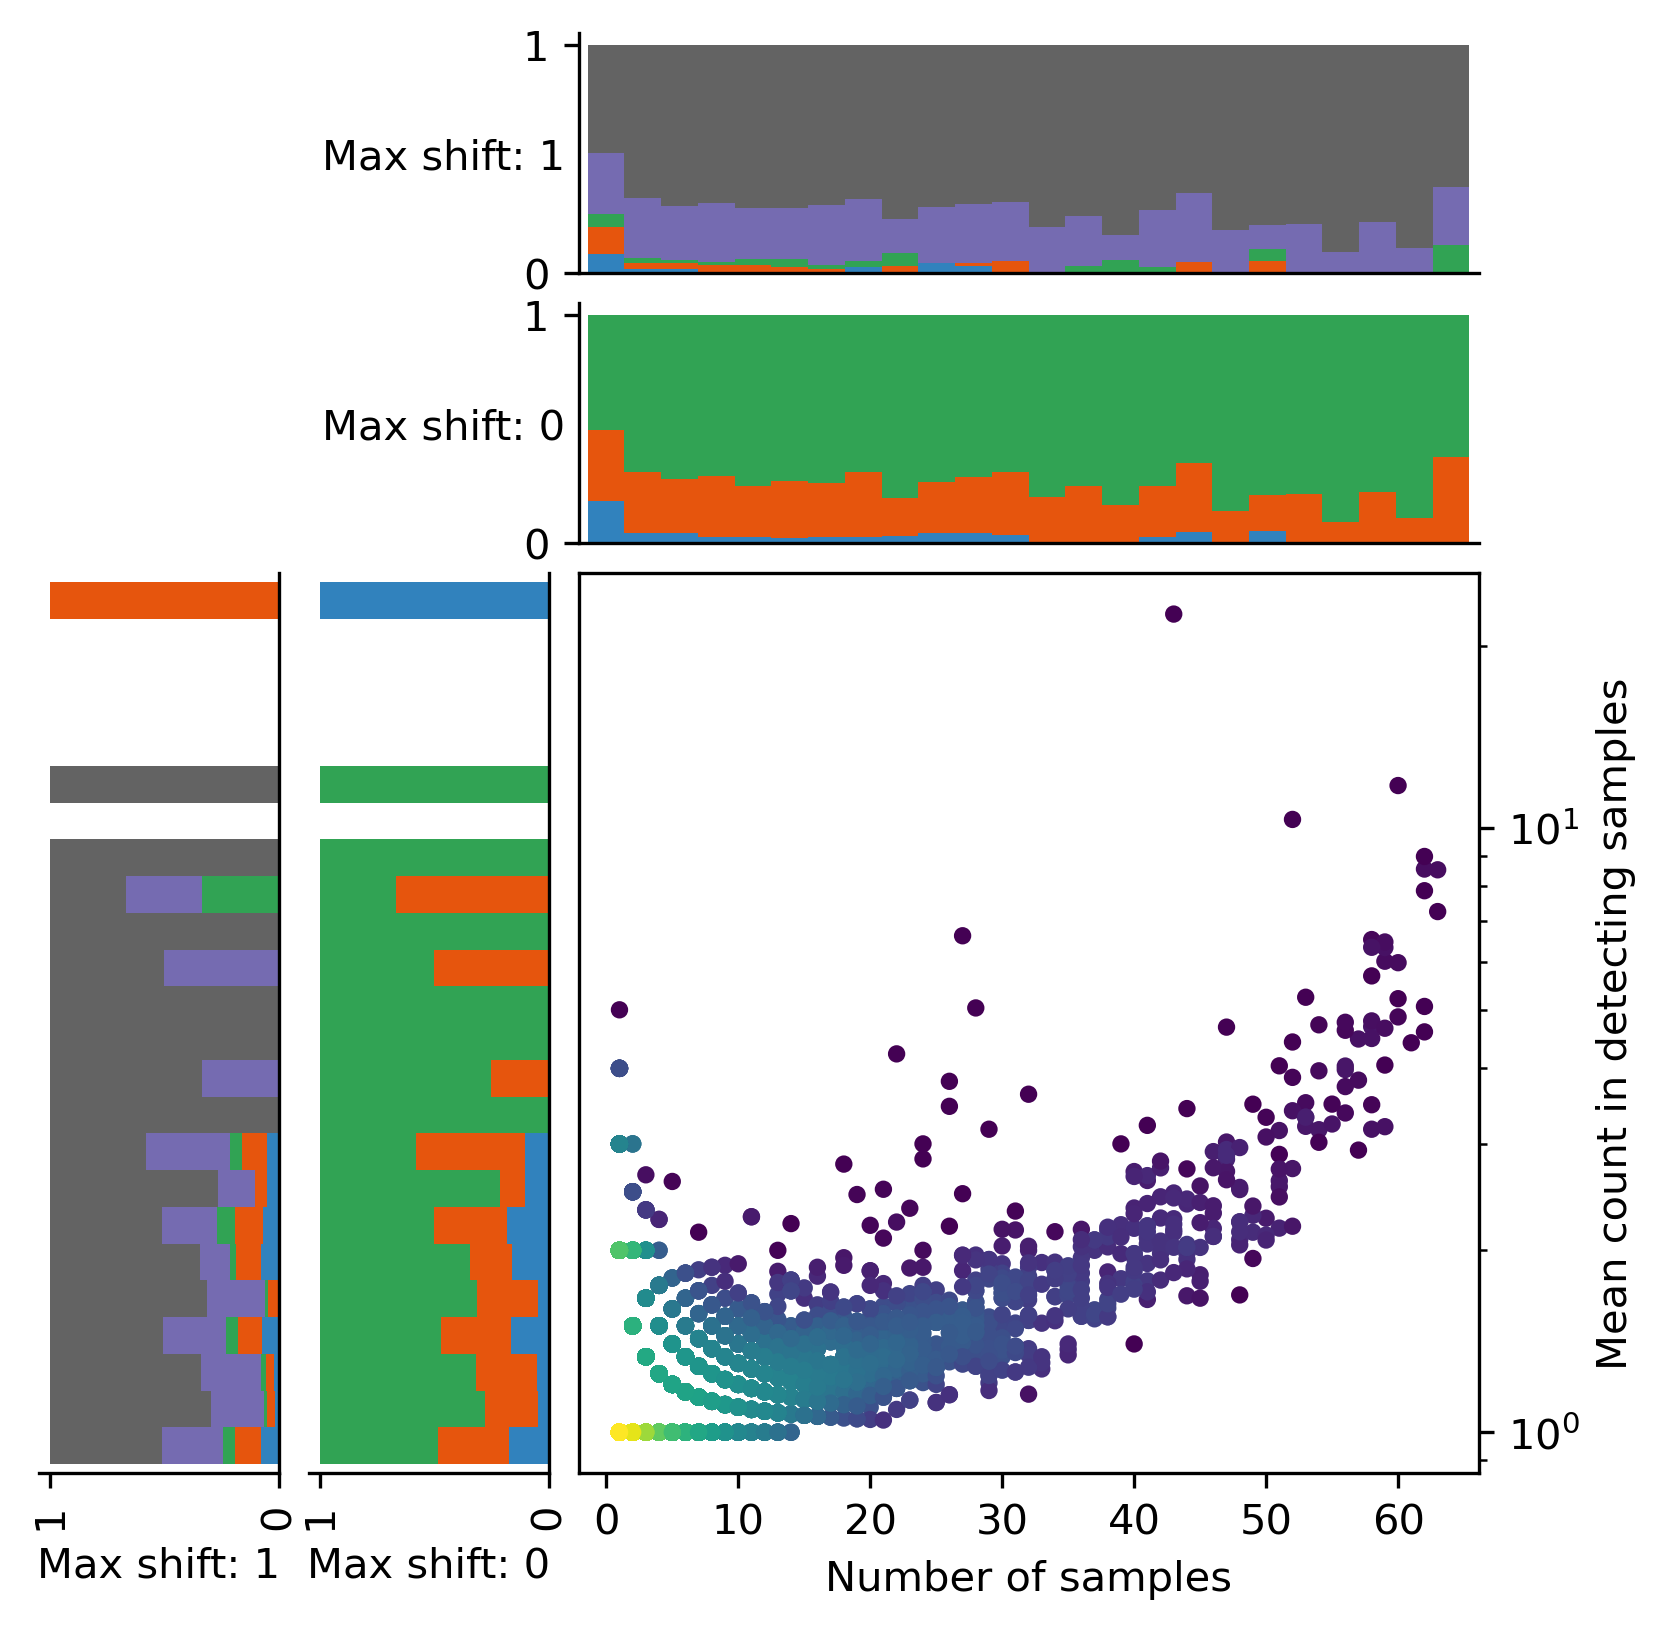
\includegraphics[width=\linewidth]{chapters/4_results_and_discussion/figures/detection/density/circexplorer2.png}
            \caption{CircExplorer2}
            \label{fig:detection_density_circexplorer2}
        \end{subfigure}
         &
        \begin{subfigure}{.5\textwidth}
            \centering

            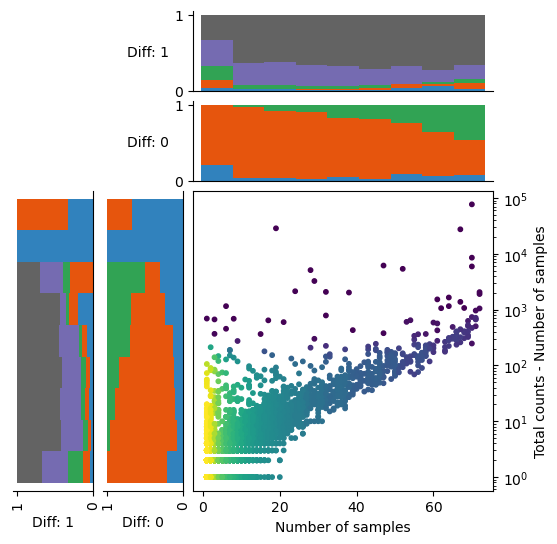
\includegraphics[width=\linewidth]{chapters/4_results_and_discussion/figures/detection/density/ciriquant.png}
            \caption{CIRI2}
            \label{fig:detection_density_ciriquant}
        \end{subfigure} \\
        \begin{subfigure}{.5\textwidth}
            \centering

            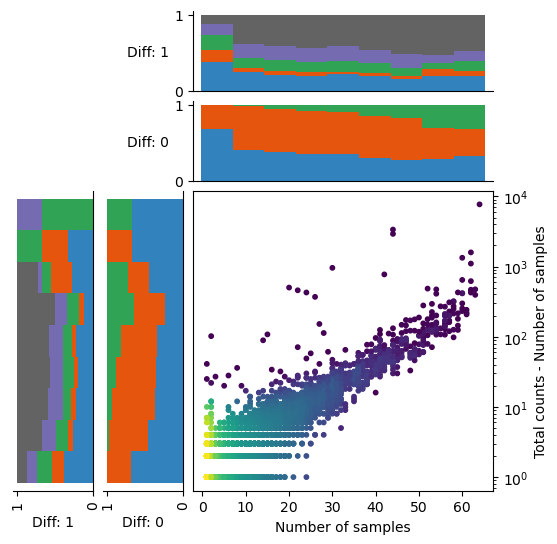
\includegraphics[width=\linewidth]{chapters/4_results_and_discussion/figures/detection/density/dcc.png}
            \caption{DCC}
            \label{fig:detection_density_dcc}
        \end{subfigure}
         &
        \begin{subfigure}{.5\textwidth}
            \centering

            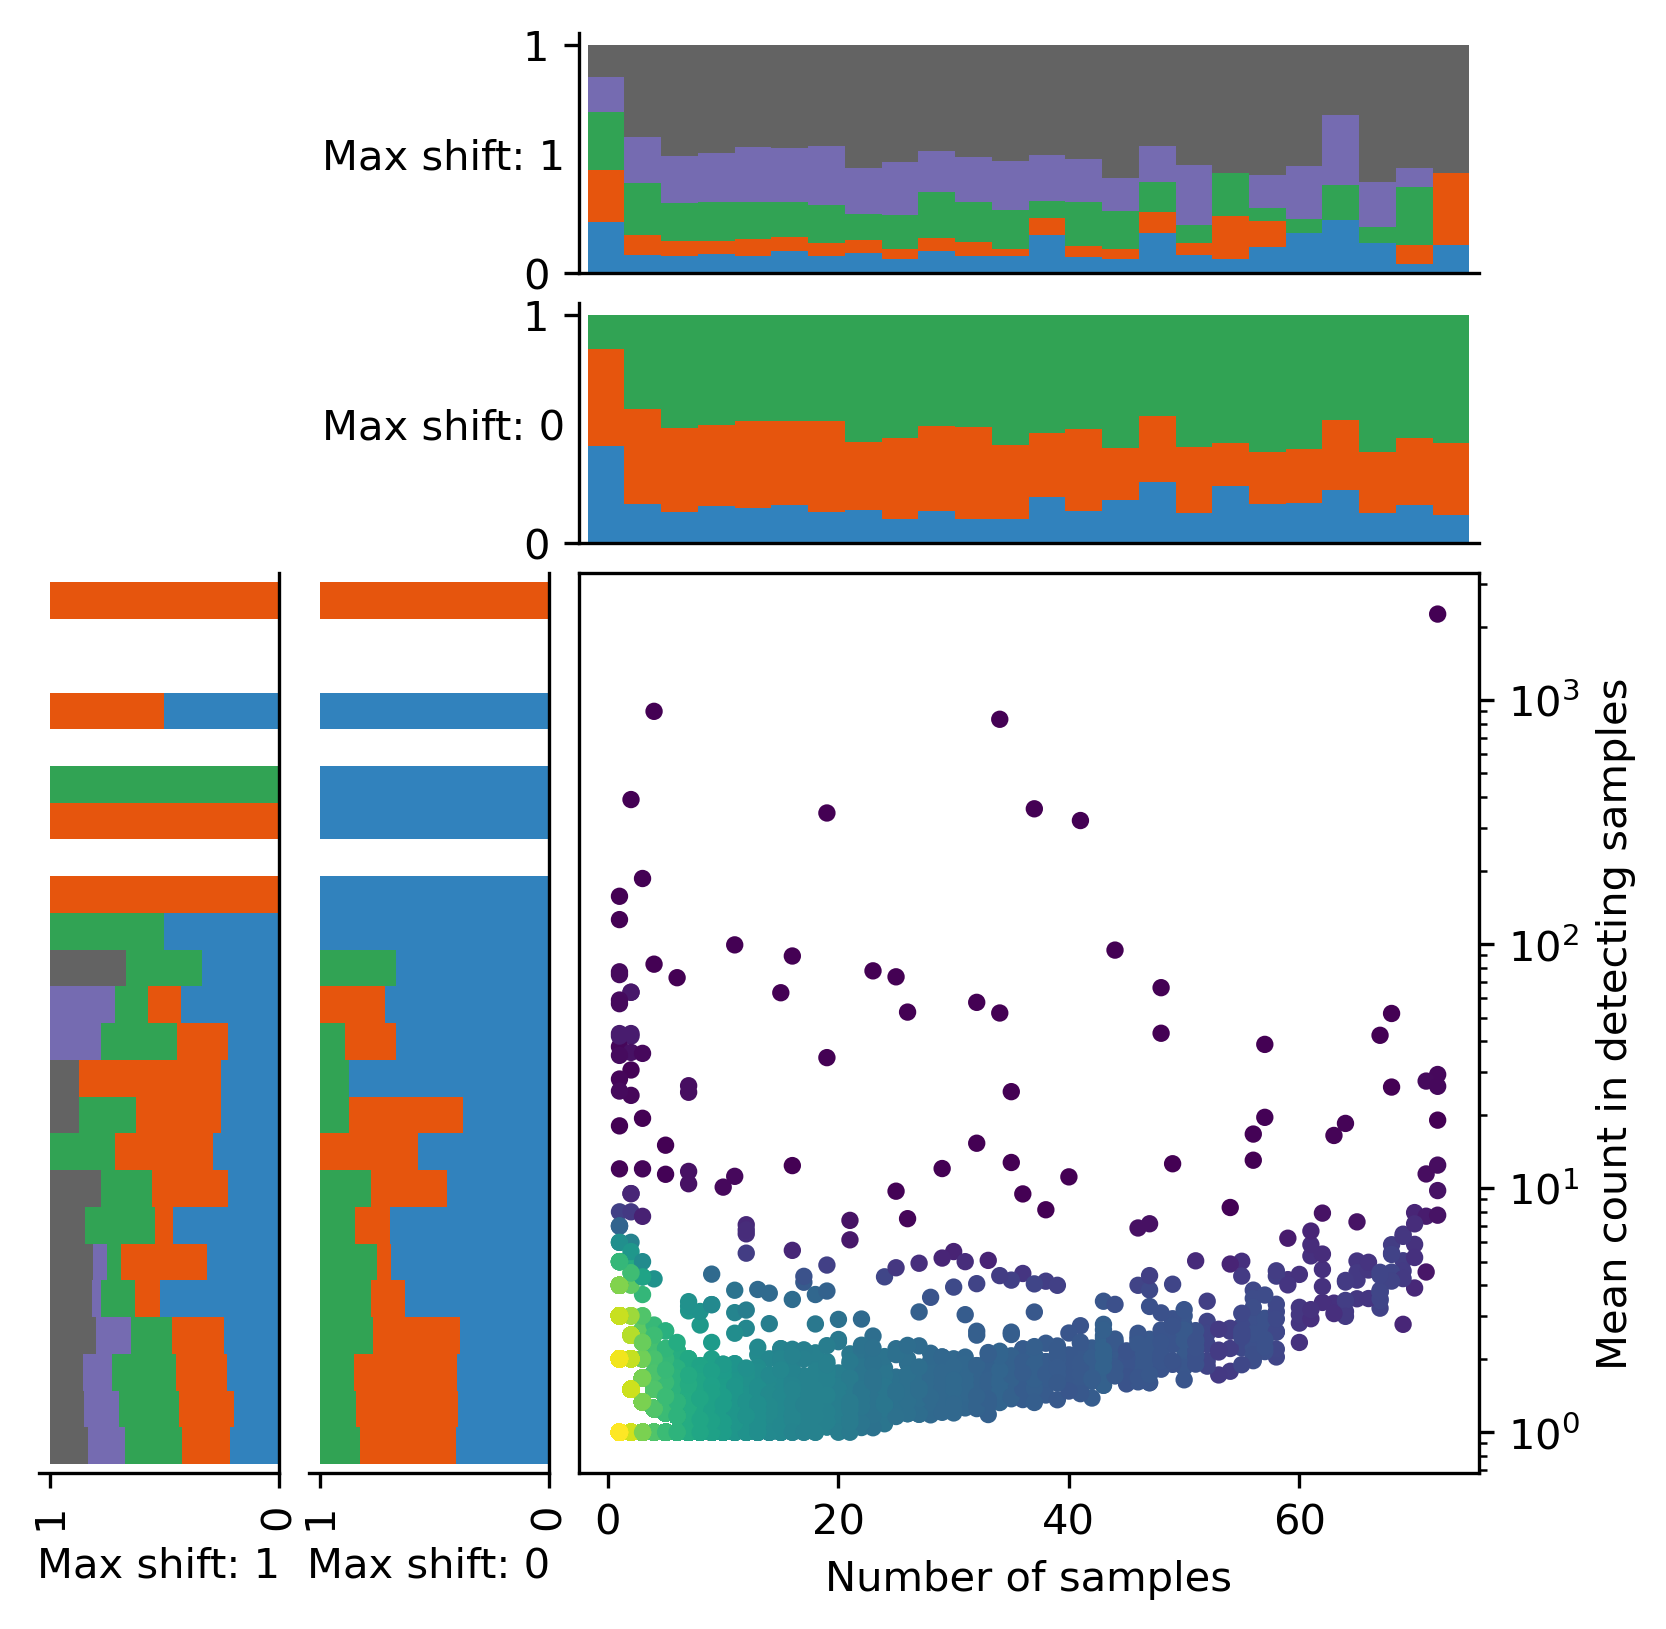
\includegraphics[width=\linewidth]{chapters/4_results_and_discussion/figures/detection/density/find_circ.png}
            \caption{find\_circ}
            \label{fig:detection_density_find-circ}
        \end{subfigure}
    \end{tabular}
    \caption{Distributions of BSJs detected by each tool.
        The x-axis shows the number of tools that detected a BSJ, while the y-axis
        shows the logarithm of the number of reads supporting the BSJ across all
        samples.
        The color indicates the density of BSJs at a given point.
        The stacked bar plots above and left of the scatter plots show the number of
        agreeing tools in the respective slice.
    }
    \label{fig:detection_density}
\end{figure}

\section{Quantification}

\begin{figure}[ht]
    \centering

    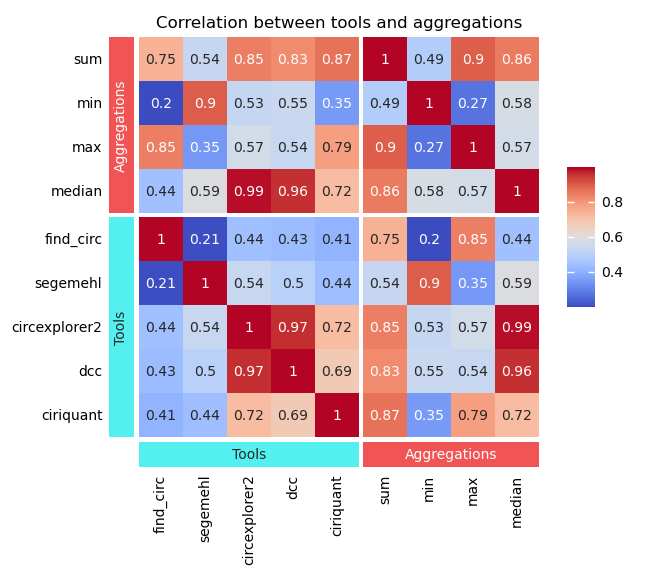
\includegraphics[width=0.7\textwidth]{chapters/4_results_and_discussion/figures/quantification/correlation_heatmap.png}
    \caption{Correlation heatmap
    }
    \label{fig:quantification_correlation_heatmap}
\end{figure}

\section{Differential expression analysis}

\section{Biological interpretation}
